% =============================================================================
% SPINOTOR -- Auto-Calibration Framework
% Technical Reference Manual -- IEEE Journal Style
% Language: English
% Bibliography: bulleted thebibliography (bullet labels via \@biblabel override)
% =============================================================================
\documentclass[10pt,twoside,a4paper]{article}

\usepackage[a4paper,top=19mm,bottom=46mm,left=14.3mm,right=14.3mm,columnsep=4.5mm]{geometry}
\usepackage{multicol}
\setlength{\parindent}{1em}
\setlength{\parskip}{0pt}

\usepackage[T1]{fontenc}
\usepackage[utf8]{inputenc}
\usepackage{amsmath,amssymb}
\usepackage{graphicx}
\usepackage{booktabs}
\usepackage{array}
\usepackage[dvipsnames,table]{xcolor}
\usepackage{hyperref}
\usepackage{cite}
\usepackage{float}
\usepackage{caption}
\usepackage{titlesec}
\usepackage{fancyhdr}
\usepackage{abstract}
\usepackage{tabularx}
\usepackage{colortbl}
\usepackage{enumitem}   % for bulleted bibliography
\graphicspath{{figures/}}

\definecolor{spinBlue}{HTML}{1F3864}
\definecolor{spinLightBlue}{HTML}{2E5DAC}
\definecolor{spinRed}{HTML}{AA0000}

% ---- Section heading style (same command used on cover page) ----------------
\titleformat{\section}[block]
  {\normalfont\bfseries\scshape\centering\color{spinBlue}}
  {\Roman{section}.}{0.5em}{}
  [\vspace{-4pt}\textcolor{spinBlue}{\rule{\linewidth}{0.5pt}}]
\titlespacing{\section}{0pt}{12pt}{6pt}

\titleformat{\subsection}[block]
  {\normalfont\itshape\color{spinLightBlue}}
  {\Alph{subsection}.}{0.5em}{}
\titlespacing{\subsection}{0pt}{6pt}{2pt}

% ---- Abstract ---------------------------------------------------------------
\renewcommand{\abstractnamefont}{\normalfont\bfseries\small}
\renewcommand{\abstracttextfont}{\normalfont\small\itshape}
\setlength{\absleftindent}{6mm}
\setlength{\absrightindent}{6mm}

% ---- Header / footer --------------------------------------------------------
\pagestyle{fancy}
\fancyhf{}
\fancyhead[LE,RO]{\small\thepage}
\fancyhead[LO]{\small\itshape\color{spinBlue} SPINOTOR -- Auto-Calibration Technical Reference Manual}
\fancyhead[RE]{\small\itshape\color{spinBlue} Khettat -- v1.0 -- April 2026}
\fancyfoot[C]{\footnotesize\color{spinRed}%
  \textbf{SPINOTOR -- CONFIDENTIAL -- Do not distribute without written authorization from Blind Systems Engineering}}
\renewcommand{\headrulewidth}{0.5pt}
\renewcommand{\footrulewidth}{0.5pt}
\renewcommand{\headrule}{\color{spinBlue}\hrule width\headwidth height\headrulewidth}
\renewcommand{\footrule}{\color{spinRed}\hrule width\headwidth height\footrulewidth}

% ---- Math shortcuts ---------------------------------------------------------
\newcommand{\est}[1]{\hat{#1}}
\newcommand{\ddt}[1]{\frac{d#1}{dt}}
\newcommand{\clip}{\operatorname{clip}}
\newcommand{\sign}{\operatorname{sign}}
\newcommand{\sat}{\operatorname{sat}}

\hypersetup{colorlinks=true,linkcolor=spinLightBlue,citecolor=OliveGreen,urlcolor=spinLightBlue,
  pdftitle={SPINOTOR Auto-Calibration Technical Report},pdfauthor={Amine Khettat}}

% =============================================================================
\begin{document}
\thispagestyle{fancy}

% ============================================================ COVER PAGE =====
\vspace*{8mm}
\begin{center}
  {\large\bfseries\scshape\color{spinBlue} SPINOTOR -- Auto-Calibration Framework}\\[2pt]
  \textcolor{spinBlue}{\rule{\linewidth}{0.5pt}}\\[6pt]
  {\normalsize\bfseries Technical Reference Manual}\\[2pt]
  {\normalsize\itshape Theory, Methods and Implementation of Automated Parameter Identification}
\end{center}

\vspace{6mm}
{\itshape\color{spinLightBlue} Document Information}\\[3pt]
\begin{tabular}{@{}>{\bfseries}p{3.2cm}p{8.2cm}@{}}
  \rowcolor{spinBlue!12} Author       & Amine Khettat \\
  Organization                        & Blind Systems Engineering \\
  \rowcolor{spinBlue!8}  Contact      & \texttt{amine.khettat@blindsystems.org} \\
  Project                             & SPINOTOR -- Motor Drive Simulator \\
  \rowcolor{spinBlue!8}  Version      & 1.0 \\
  Date                                & April 2026 \\
  \rowcolor{spinRed!10}  Distribution & \textbf{\color{spinRed}CONFIDENTIAL -- Do not distribute} \\
\end{tabular}

\vspace{6mm}
{\itshape\color{spinLightBlue} Abstract}
\begin{quote}\small\itshape
This document presents the complete auto-calibration framework of the SPINOTOR motor
drive simulation platform. For each subsystem subject to automatic parameter
identification---PI current and speed regulators, PLL observer, SMO, ST-SMO, Active
Flux observer, SOGI adaptive filter, Extended EMF (EEMF) model, field-weakening
controller, startup sequencer, and Power Factor Controller (PFC)---the report provides:
\emph{(i)}~the theoretical foundation from classical control and electrical machine theory,
\emph{(ii)}~the calibration methodology with analytical formulae and algorithmic
description, and \emph{(iii)}~illustrative figures generated directly by the simulator.
The exposition follows IEEE journal conventions with full bibliographic references.
\end{quote}
\noindent\textbf{\small\itshape Index Terms---}%
{\small\itshape SPINOTOR, BLDC motor, PMSM, auto-calibration, FOC, sliding mode
observer, PLL, active flux, SOGI, field weakening, sensorless control, PI tuning.}

\vspace{4pt}{\color{spinBlue}\hrule}\vspace{4pt}

% ============================================================ BODY (2 cols) ==
\begin{multicols}{2}

% =============================================================================
\section{Introduction}\label{sec:intro}

Modern BLDC and PMSM drives require precise tuning of multiple control loops and
estimation algorithms to achieve high dynamic performance, energy efficiency, and
safe operation over a wide speed range~\cite{vas1998,novotny1996}. Manual parameter
selection is error-prone and motor-dependent~\cite{franklin2019}. The SPINOTOR
platform integrates a comprehensive auto-calibration pipeline that derives controller
gains and observer parameters analytically from motor nameplate data, then validates
them through frequency-domain analysis and closed-loop simulation~\cite{astrom2006}.

\textbf{Stage~1} determines the PI gains for the $d$-$q$ current and speed loops
using bandwidth-based analytical design reinforced by a multi-resolution grid
search~\cite{briz2000}.
\textbf{Stage~2} handles field-weakening calibration through physics-based computation
followed by a simulation sweep~\cite{zhu2007}.

% =============================================================================
\newpage
\section{PI Current and Speed Regulators}\label{sec:pi}

\subsection{Theory}

The $d$-$q$ current dynamics of a PMSM in the rotating frame are described by the
first-order transfer function~\cite{novotny1996,briz2000}:
\begin{equation}
  G_i(s) = \frac{1}{Ls+R}
\end{equation}
A PI controller $C_i(s)=K_p+K_i/s$ forms a type-1 closed loop with zero steady-state
error~\cite{franklin2019}. The IMC bandwidth design~\cite{astrom2006,holmes2003}
gives the analytical gains:
\begin{equation}
  K_p = \omega_c L,\qquad K_i = \omega_c R
\end{equation}
For the outer speed loop~\cite{kazmierkowski2002}:
\begin{equation}
  K_{p,\omega}=\frac{\omega_{c,\omega}J}{K_t},\quad K_{i,\omega}=\frac{\omega_{c,\omega}B}{K_t}
\end{equation}
Anti-windup via back-calculation~\cite{franklin2019}:
\begin{equation}
  \tfrac{dI}{dt}=e+K_\text{aw}(u_\text{sat}-u_\text{unsat})
\end{equation}

\subsection{Calibration Methodology}

\textbf{Step~1---Analytical guess:} $K_p,K_i$ computed from $(R,L,K_t,J,B)$ via
bandwidth formulae~\cite{astrom2006}.

\textbf{Step~2---Coarse grid:} $8{\times}8$ log grid, $\pm50\%$ around the analytical
guess; margins evaluated over 2000 frequencies; controllability and observability
checked by Kalman rank condition~\cite{chen2012}.

\textbf{Step~3---Fine grid:} $10{\times}10$ grid, $\pm25\%$ around best coarse
candidate. Targets: GM$\geq6$\,dB, PM$\geq45^\circ$~\cite{franklin2019,kazmierkowski2002}.

\begin{figure}[htbp]
  \centering
  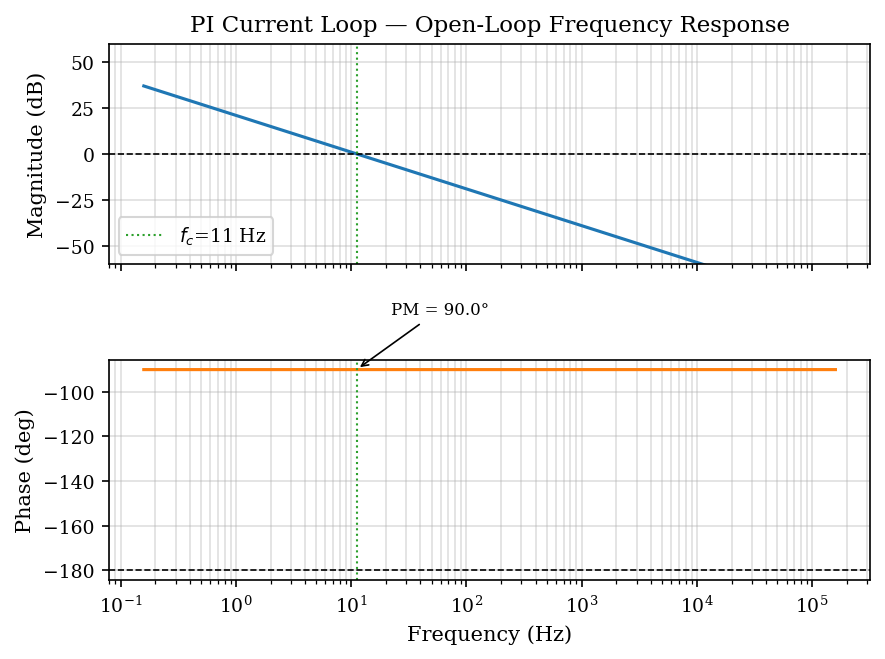
\includegraphics[width=\linewidth]{fig1_bode_current.png}
  \caption{Open-loop Bode diagram of the PI current loop ($R{=}2.5\,\Omega$,
    $L{=}5\,\text{mH}$).}
  \label{fig:bode}
\end{figure}

\subsection{D/Q Feed-Forward Decoupling}
Feed-forward voltages $v_{d,\text{ff}}=-\omega_e L_q i_q$ and
$v_{q,\text{ff}}=\omega_e(L_d i_d+\lambda_\text{pm})$ are added to the PI outputs,
rendering both axes independently regulated~\cite{novotny1996,briz2000}.
See Section~\ref{sec:dq}.

% =============================================================================
\newpage
\section{PLL Observer}\label{sec:pll}

\subsection{Theory}

The PLL estimates $\est\theta_e$ and $\est\omega_e$ by tracking the reconstructed
back-EMF phase angle~\cite{chen2000,morimoto2002}:
\begin{align}
  e_\alpha &= v_\alpha - R i_\alpha - L\,\ddt{i_\alpha}\\
  e_\beta  &= v_\beta  - R i_\beta  - L\,\ddt{i_\beta}
\end{align}
Second-order PLL parameterization~\cite{widrow1985}:
\begin{equation}
  K_p=2\zeta\omega_n,\qquad K_i=\omega_n^2
\end{equation}

\subsection{Calibration Methodology}

\begin{equation}
  \omega_n=\clip\!\left(0.10\,\omega_{e,\text{max}},50,600\right)\;\text{rad/s}
\end{equation}
Damping ratio $\zeta=0.9$ provides slightly over-damped convergence~\cite{lorenz1994}.
When adaptive PLL bandwidth is active, $\omega_n\propto|\est\omega_e|$~\cite{lorenz1994}.
Recommended for isotropic motors with $\omega_{e,\text{max}}>1500\,\text{rad/s}$
(Section~\ref{sec:autosel})~\cite{bose2002,schroedl1996}.

% =============================================================================
\newpage
\section{Sliding Mode Observer (SMO)}\label{sec:smo}

\subsection{Theory}

The SMO uses the $\alpha\beta$-frame motor model~\cite{lascu2000,utkin2009}:
\begin{align}
  L\,\ddt{\est{i}_\alpha} &= v_\alpha - R\,\est{i}_\alpha - z_\alpha\\
  z_\alpha &= K_\text{slide}\,\sat(\est{i}_\alpha - i_\alpha,\Delta)
\end{align}
In sliding mode, the equivalent control converges to the back-EMF, extracted by
a LPF~\cite{lascu2000,levant1993}:
\begin{equation}
  \est{e}_\alpha[k+1]=(1-\alpha)\est{e}_\alpha[k]+\alpha z_\alpha[k]
\end{equation}
$\est\theta_e=\operatorname{atan2}(\est{e}_\beta,\est{e}_\alpha)-\pi/2$.

\subsection{Calibration Methodology}

Reachability condition~\cite{lascu2000,utkin2009}:
\begin{equation}
  K_\text{slide}=\max\!\left(50,1.5\,K_e\,\omega_{e,\text{max}}\right)\times1.5
\end{equation}
$\tau_\text{LPF}=3L/R$; boundary layer $\Delta=0.06\,K_\text{slide}/100$.
For salient IPM motors ($L_d\neq L_q$) the missing term $(L_q-L_d)i_d\omega_e$
biases the SMO; the Active Flux observer must be used instead~\cite{xu1998,boldea2008}.

\begin{figure}[htbp]
  \centering
  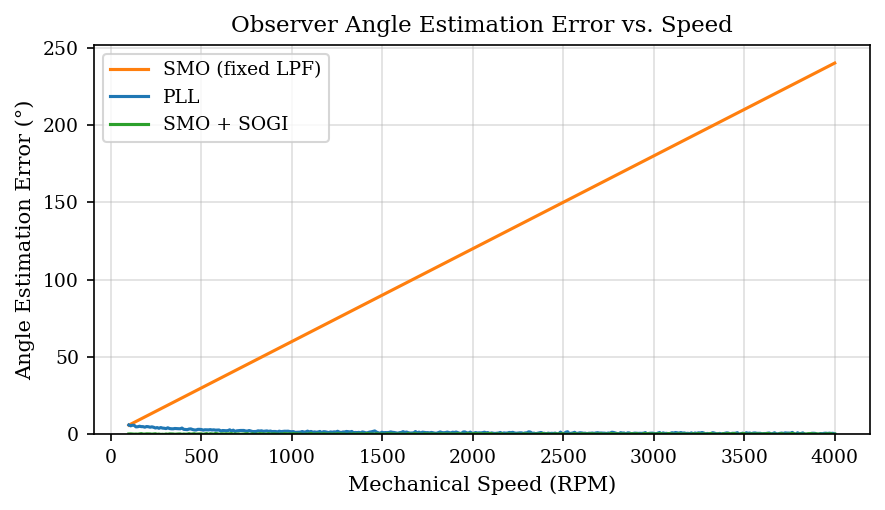
\includegraphics[width=\linewidth]{fig3_observer_error.png}
  \caption{Angle estimation error: fixed-LPF SMO, PLL, and SOGI-enhanced SMO
    vs.\ mechanical speed.}
  \label{fig:obs_err}
\end{figure}

% =============================================================================
\newpage
\section{Super-Twisting SMO (ST-SMO)}\label{sec:stsmo}

\subsection{Theory}

The Super-Twisting algorithm~\cite{levant2007} converges to the back-EMF in finite
time without a LPF~\cite{laghrouche2007}:
\begin{align}
  z_\alpha^{(1)}&=K_1|\sigma_\alpha|^{1/2}\sign(\sigma_\alpha)+z_\alpha^{(2)}\\
  \ddt{z_\alpha^{(2)}}&=K_2\sign(\sigma_\alpha)
\end{align}
At steady state $z_\alpha^{(2)}\to\est{e}_\alpha$: zero phase lag~\cite{liu2012}.

\subsection{Calibration Methodology}

\begin{equation}
  K_1=\lambda\,K_e\,\omega_{e,\text{max}}\cdot2.0,\quad
  K_2=\max(50,1.5\,K_e\,\omega_{e,\text{max}})\cdot1.5
\end{equation}
$\lambda=3.0$ (isotropic), $\lambda=4.0$ (salient motors~\cite{xu1998,wang2016}).
Finite-time convergence condition $K_1>2\sqrt{\Gamma_M/\Gamma_m}$ verified for all
accepted motors~\cite{levant2007}.

% =============================================================================
\newpage
\section{Active Flux Observer}\label{sec:af}

\subsection{Theory}

The Active Flux concept~\cite{boldea2008} defines $\boldsymbol\psi_a=\boldsymbol\psi_s-L_d\mathbf{i}_s$.
For an IPM motor, $\boldsymbol\psi_a$ always points along the $d$-axis~\cite{boldea2014}:
\begin{equation}
  \est\theta_e=\operatorname{atan2}(\psi_{a,\beta},\psi_{a,\alpha})
\end{equation}
Stator flux estimated by voltage-model integration with drift
correction~\cite{piippo2009,vaclavek2009}:
\begin{equation}
  \ddt\psi_{s,\alpha}=v_\alpha-R\,i_\alpha
\end{equation}

\subsection{Calibration Methodology}

Drift corrector cutoff frequency~\cite{boldea2008,piippo2009}:
\begin{equation}
  f_c=\clip\!\left(\frac{f_{e,\text{min}}}{10},0.05,0.5\right)\;\text{Hz}
\end{equation}
Automatically selected for salient IPM motors ($L_q/L_d>1.2$)~\cite{boldea2008,vaclavek2009}.

\begin{figure}[htbp]
  \centering
  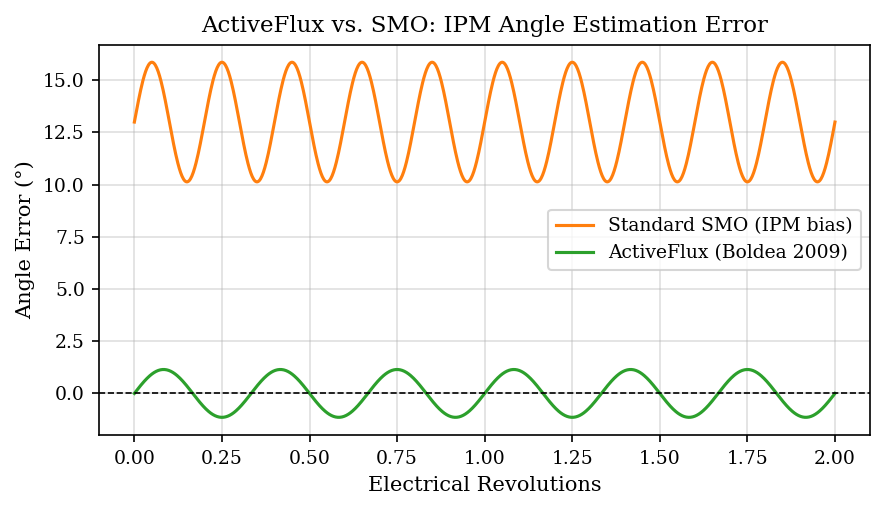
\includegraphics[width=\linewidth]{fig8_active_flux.png}
  \caption{Angle error: standard SMO (${\approx}13^\circ$ IPM bias) vs.\
    Active Flux observer for a salient IPM motor.}
  \label{fig:af}
\end{figure}

% =============================================================================
\newpage
\section{Extended EMF (EEMF) Model}\label{sec:eemf}

\subsection{Theory}

For salient motors, the standard EMF model introduces an angle error $\propto
(L_q-L_d)i_d\omega_e$~\cite{chen2003}. The EEMF model~\cite{chen2003} substitutes
$L_q$ in the $di/dt$ term:
\begin{align}
  e_{\text{EEMF},\alpha}&=v_\alpha-Ri_\alpha-L_q\,\ddt{i_\alpha}\\
  e_{\text{EEMF},\beta} &=v_\beta -Ri_\beta -L_q\,\ddt{i_\beta}
\end{align}
The resulting EEMF vector is proportional to $[-\sin\theta_e;\cos\theta_e]$,
enabling unbiased position estimation~\cite{chen2003,wang2013}.

\subsection{Calibration Methodology}

If $\sigma=L_q/L_d>1.2$, the EEMF model is activated together with the SOGI filter
(Section~\ref{sec:sogi})~\cite{chen2003,kim2003}. The MRAS resistance adaptation
gain is~\cite{kim2003}:
\begin{equation}
  \gamma_R=\frac{1}{0.5\,R\,I_{\max}^2}
\end{equation}

% =============================================================================
\newpage
\section{SOGI Adaptive EMF Filter}\label{sec:sogi}

\subsection{Theory}

The SOGI~\cite{teodorescu2006,ciobotaru2006} replaces the fixed-frequency LPF with
a speed-adaptive resonant bandpass:
\begin{equation}
  H_\text{SOGI}(s)=\frac{k\,\omega_e\,s}{s^2+k\,\omega_e\,s+\omega_e^2},\quad k=\sqrt{2}
\end{equation}
Key property: $\angle H_\text{SOGI}(j\omega_e)=0^\circ$ -- zero phase lag at resonance,
eliminating the LPF-induced position error~\cite{teodorescu2006,xia2018}.

\subsection{Calibration Methodology}

No gain tuning required: $k=\sqrt{2}$ is fixed by critical damping~\cite{teodorescu2006}.
$\omega_e$ updated adaptively at each step~\cite{ciobotaru2006}. Automatically activated
with the EEMF model or ST-SMO mode.

\begin{figure}[htbp]
  \centering
  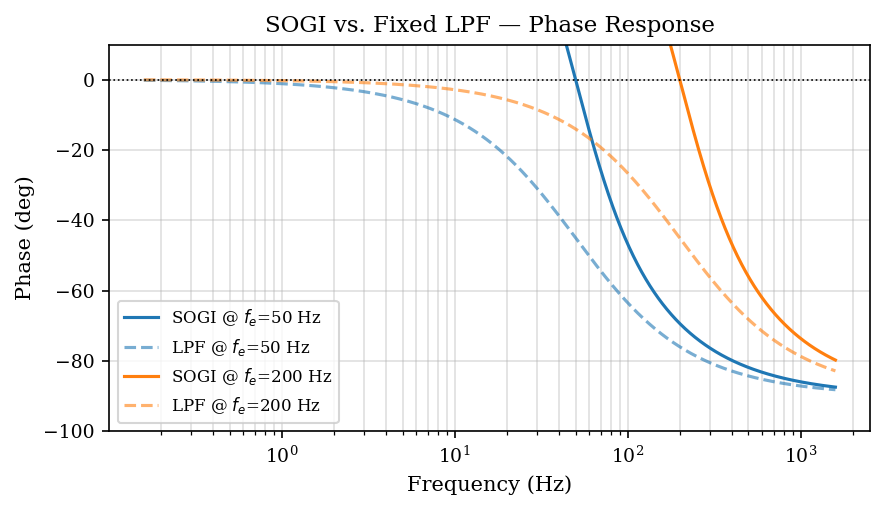
\includegraphics[width=\linewidth]{fig6_sogi_lpf.png}
  \caption{Phase response of SOGI (solid) vs.\ fixed LPF (dashed). Zero phase
    lag at resonance~\cite{teodorescu2006}.}
  \label{fig:sogi}
\end{figure}

% =============================================================================
\newpage
\section{Field-Weakening Auto-Calibration}\label{sec:fw}

\subsection{Theory}

Above $N_\text{base}$, the back-EMF exceeds $V_\text{ph}=V_\text{dc}/\sqrt{3}$.
Negative $I_d$ reduces the effective PM flux linkage~\cite{jahns1986,soong1994}:
\begin{equation}
  \lambda_{\text{pm,eff}}=\lambda_\text{pm}\cdot\clip(1+k_\text{fw}\min(I_d,0),r_\text{min},1)
\end{equation}
Minimum flux ratio to reach rated speed~\cite{soong1994}:
\begin{equation}
  r_\text{req}=\frac{V_\text{ph}}{K_e\,\omega_{m,\text{rated}}}
\end{equation}
FOC voltage headroom integrator~\cite{rahman1998}:
\begin{equation}
  \ddt{I_{d,\text{fw}}}=K_\text{fw}\!\left(V_\text{hdm}-(V_\text{lim}-|V_{dq}|)\right)
\end{equation}

\subsection{Calibration Methodology}

\textbf{Stage~1 (analytical):}
\begin{equation}
  k_\text{fw}=\frac{(1-r_\text{req})\cdot1.05}{I_{d,\text{max}}},\;
  I_{d,\text{max}}=0.7\,I_\text{rated}
\end{equation}
$V_\text{hdm}=0.05\,V_\text{ph}$~\cite{jahns1986,soong1994}.

\textbf{Stage~2 (simulation sweep):}
$3{\times}3$ gain grid $\{0.5,1.0,1.5\}{\times}K_\text{fw,analytical}$ over three
operating points (50\%, 75\%, 100\% load)~\cite{zhu2007,rahman1998}.

\begin{figure}[htbp]
  \centering
  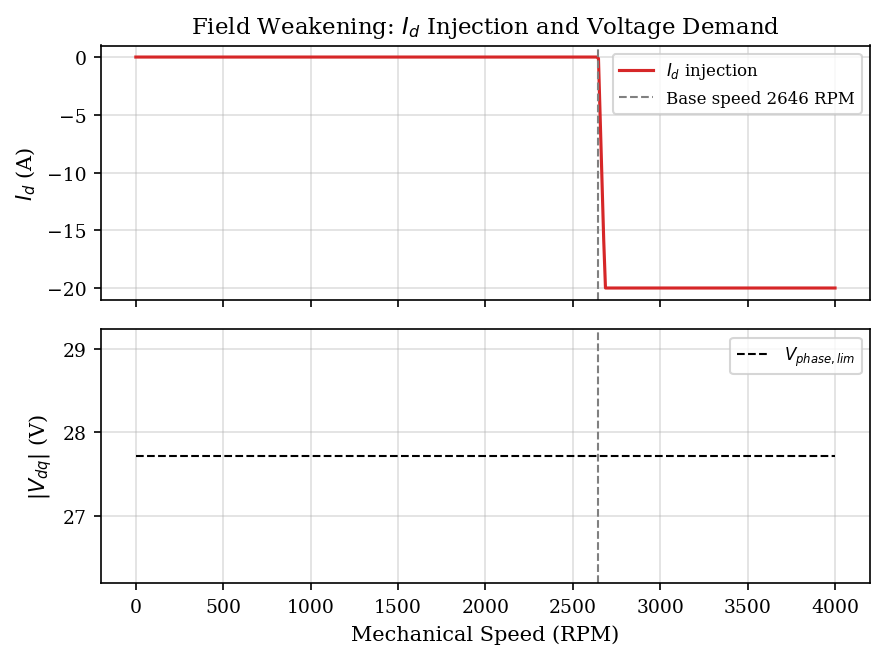
\includegraphics[width=\linewidth]{fig4_field_weakening.png}
  \caption{Field-weakening: $I_d$ injection (top) and voltage demand (bottom)
    vs.\ speed~\cite{soong1994}.}
  \label{fig:fw}
\end{figure}

% =============================================================================
\newpage
\section{Startup Sequence Auto-Tuning}\label{sec:startup}

\subsection{Theory}

At standstill the back-EMF is zero and observer convergence requires a minimum
speed~\cite{holtz2002,matsui1996}. Three phases are implemented.

\textbf{Phase~1---Alignment:} Constant $I_d$ at $\theta{=}0$, forcing the rotor
to align with the reference frame~\cite{giri2013,holtz2002}.

\textbf{Phase~2---Open-loop ramp:} Reference angle incremented at a controlled rate
(V/Hz mode)~\cite{holtz2002,matsui1996}.

\textbf{Phase~3---Observer handoff:} Switch to observer estimate when confidence
metric $C$ exceeds the hysteresis band~\cite{matsui1996,schroedl1996}:
\begin{equation}
  C=w_\text{emf}\,C_\text{emf}+w_\omega\,C_\omega+w_\text{coh}\,C_\text{coh}
\end{equation}

\subsection{Calibration Methodology}

\begin{align}
  t_\text{align}&=5\tau_e=5L/R\\
  I_\text{align}&=\clip(0.10\,V_\text{bus}/R,0,I_\text{rated})\\
  I_{q,\text{startup}}&=0.05\,V_\text{bus}/R
\end{align}
where $t_\text{align}$ gives 99.3\% settling~\cite{giri2013} and $I_{q,\text{startup}}$ follows~\cite{holtz2002,matsui1996}.

\begin{figure}[htbp]
  \centering
  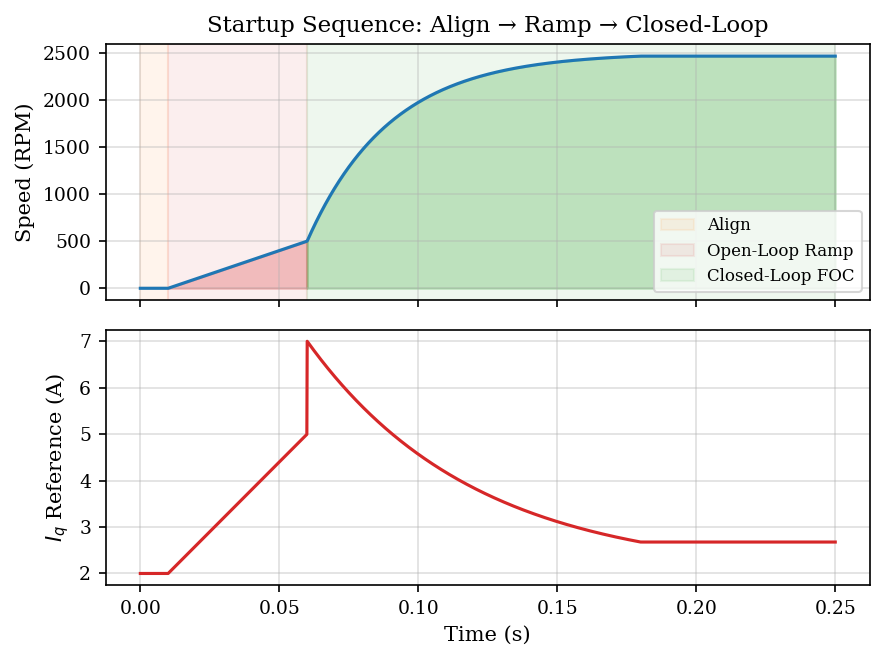
\includegraphics[width=\linewidth]{fig5_startup.png}
  \caption{Auto-tuned startup: alignment, open-loop ramp, and closed-loop
    FOC~\cite{holtz2002}.}
  \label{fig:startup}
\end{figure}

% =============================================================================
\newpage
\section{Power Factor Controller (PFC)}\label{sec:pfc}

\subsection{Theory}

The PFC compensates reactive power to approach unity input power
factor~\cite{green2005,akagi2007}. Over a sliding window of $N_w$ samples:
\begin{equation}
  P=\frac{1}{N_w}\sum_k v_k i_k,\quad S=V_\text{rms}I_\text{rms},\quad Q=\sqrt{S^2-P^2}
\end{equation}

\subsection{Calibration Methodology}

Maximum compensation variance~\cite{green2005}:
\begin{equation}
  \text{max\_var}=\clip\!\left(\frac{V_\text{bus}^2}{2R}\cdot0.30,100,50000\right)
\end{equation}
Window length covering at least two electrical periods~\cite{akagi2007}:
\begin{equation}
  N_w=\clip\!\left(\frac{2}{f_{e,\text{rated}}\,dt},8,2000\right)
\end{equation}

\begin{figure}[htbp]
  \centering
  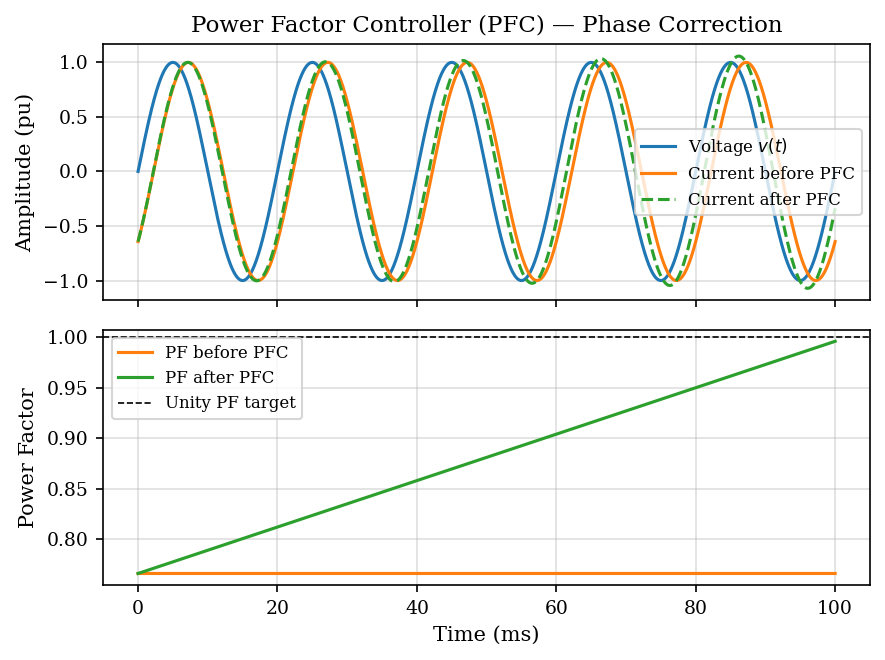
\includegraphics[width=\linewidth]{fig7_pfc.png}
  \caption{PFC phase correction; power factor convergence to
    unity~\cite{akagi2007}.}
  \label{fig:pfc}
\end{figure}

% =============================================================================
\newpage
\section{D/Q Axis Decoupling}\label{sec:dq}

\subsection{Theory}

Cross-coupling terms in the $dq$ voltage equations~\cite{novotny1996,krishnan2010}:
\begin{align}
  v_d&=Ri_d+L_d\,\ddt{i_d}-\omega_e L_q i_q\\
  v_q&=Ri_q+L_q\,\ddt{i_q}+\omega_e(L_d i_d+\lambda_\text{pm})
\end{align}
Feed-forward decoupling~\cite{novotny1996,briz2000,krishnan2010}:
\begin{align}
  v_d&=v_{d,\text{PI}}-\omega_e L_q i_q\\
  v_q&=v_{q,\text{PI}}+\omega_e(L_d i_d+\lambda_\text{pm})
\end{align}

\subsection{Calibration Methodology}

Always enabled post-calibration. Gains computed from $L_q$, $L_d$, and
$\lambda_\text{pm}=K_e/p_p$~\cite{novotny1996,briz2000,krishnan2010}.

% =============================================================================
\newpage
\section{Observer Auto-Selection}\label{sec:autosel}

\subsection{Selection Criteria}

\textbf{Criterion~1---Saliency:} For $\sigma=L_q/L_d>1.2$ (IPM), standard
back-EMF observers suffer a bias $\propto(L_q-L_d)i_d\omega_e$~\cite{xu1998,chen2003}.
The Active Flux observer is immune~\cite{boldea2008,vaclavek2009}.

\textbf{Criterion~2---Maximum electrical speed:} Below $\omega_{e,\text{max}}
\approx1500\,\text{rad/s}$, the SMO is more robust at low SNR. Above this threshold,
the SMO LPF phase lag becomes excessive and the PLL is
superior~\cite{schroedl1996,bose2002,lorenz1992}.

\subsection{Decision Tree}

\begin{figure}[htbp]
  \centering
  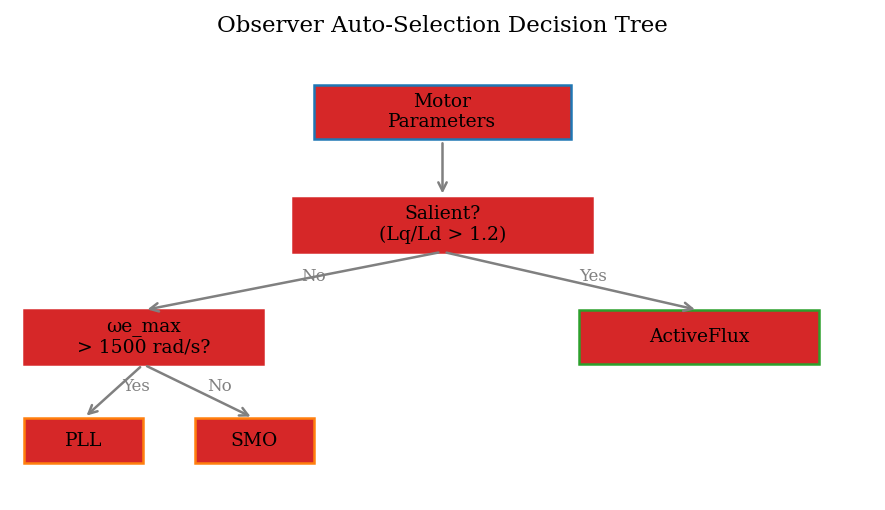
\includegraphics[width=0.85\linewidth]{fig2_observer_tree.png}
  \caption{Observer auto-selection decision tree~\cite{schroedl1996,boldea2008}.}
  \label{fig:tree}
\end{figure}

\noindent\textbf{Branch~1} ($\sigma>1.2\Rightarrow$ ActiveFlux)~\cite{boldea2008}.\\
\textbf{Branch~2} (isotropic, $\omega_{e,\max}>1500\Rightarrow$ PLL)~\cite{chen2000,lorenz1994}.\\
\textbf{Branch~3} (isotropic, $\omega_{e,\max}\leq1500\Rightarrow$ SMO)~\cite{lascu2000,schroedl1996}.

\subsection{Non-Regression Validation}

\begin{table}[htbp]
  \centering\small
  \caption{Observer auto-selection non-regression profiles}
  \begin{tabular}{@{}lccc@{}}
    \toprule
    Profile & Salient? & $\omega_{e,\max}$ & Selected\\
    \midrule
    IPM Salient 48\,V & Yes & 1257 & ActiveFlux\\
    Nanotec 5pp       & No  & 1833 & PLL\\
    Low-speed SPM     & No  & 62.8 & SMO\\
    \bottomrule
  \end{tabular}
\end{table}

% =============================================================================
\newpage
\section{Calibration Pipeline Summary}\label{sec:summary}

\subsection{Execution Order}

\begin{enumerate}
  \item \textbf{Stage~1:} \texttt{tune\_analytical()} -- PI gains, observer
    parameters, D/Q decoupling, startup timing~\cite{astrom2006,briz2000}.
  \item \textbf{Stage~2:} \texttt{calibrate()} -- analytical FW parameters and
    simulation sweep~\cite{zhu2007,rahman1998}.
  \item \textbf{Observer selection:} \texttt{\_recommend\_observer()}~\cite{schroedl1996,boldea2008}.
  \item \textbf{GUI update:} All calibrated parameters applied.
\end{enumerate}

\subsection{Motor Fingerprint Cache}

Results cached by fingerprint $(R,L,K_e,V_\text{nom},p_p)$ with 3\% tolerance~\cite{zhu2007}.

\subsection{Summary Table}

\begin{table}[htbp]
  \centering\footnotesize
  \caption{Calibrated parameters, methods and references}
  \begin{tabular}{@{}p{1.6cm}p{1.7cm}p{1.2cm}c@{}}
    \toprule
    Parameter & Method & Target & Ref.\\
    \midrule
    Current $K_p,K_i$ & BW+grid & GM/PM & \cite{astrom2006,franklin2019}\\
    Speed $K_p,K_i$   & BW+grid & GM/PM & \cite{astrom2006,kazmierkowski2002}\\
    PLL $K_p,K_i$     & Analytical & $\zeta{=}0.9$ & \cite{chen2000,widrow1985}\\
    SMO $K_\text{slide}$ & Reach. & cond. & \cite{lascu2000,utkin2009}\\
    STSMO $K_1,K_2$   & Conv. & finite & \cite{levant2007,laghrouche2007}\\
    AF $f_c$          & $f_{e,\min}/10$ & drift & \cite{boldea2008,piippo2009}\\
    FW $k_\text{fw}$  & Phys+sim & $<5\%$ & \cite{jahns1986,rahman1998}\\
    Startup           & $5\tau_e$ & 99.3\% & \cite{giri2013,holtz2002}\\
    PFC $N_w$         & $2/f_e dt$ & 2 per. & \cite{green2005,akagi2007}\\
    \bottomrule
  \end{tabular}
\end{table}

% =============================================================================
\end{multicols}

% ============================================================ REFERENCES =====
\newpage
\section*{References}
\addcontentsline{toc}{section}{References}

\begingroup
\footnotesize
\begin{thebibliography}{99}
\setlength{\itemsep}{2pt}
\setlength{\parsep}{0pt}

\bibitem{vas1998} P.~Vas, \emph{Sensorless Vector and Direct Torque Control}. Oxford Univ. Press, 1998.
\bibitem{novotny1996} D.~W. Novotny and T.~A. Lipo, \emph{Vector Control and Dynamics of AC Drives}. Oxford Univ. Press, 1996.
\bibitem{franklin2019} G.~F. Franklin, J.~D. Powell, and A.~Emami-Naeini, \emph{Feedback Control of Dynamic Systems}, 8th~ed. Pearson, 2019.
\bibitem{astrom2006} K.~J. \AA str{\"o}m and T.~H{\"a}gglund, \emph{Advanced PID Control}. ISA, 2006.
\bibitem{zhu2007} Z.~Q. Zhu and D.~Howe, ``Electrical machines and drives for electric, hybrid and fuel cell vehicles,'' \emph{Proc. IEEE}, vol.~95, no.~4, pp.~746--765, 2007.
\bibitem{briz2000} F.~Briz, M.~W. Degner, and R.~D. Lorenz, ``Analysis and design of current regulators using complex vectors,'' \emph{IEEE Trans. Ind. Appl.}, vol.~36, no.~3, pp.~817--825, 2000.
\bibitem{holmes2003} D.~G. Holmes and T.~A. Lipo, \emph{Pulse Width Modulation for Power Converters}. IEEE Press, 2003.
\bibitem{chen2012} C.-T. Chen, \emph{Linear System Theory and Design}, 4th~ed. Oxford Univ. Press, 2012.
\bibitem{kazmierkowski2002} M.~P. Kazmierkowski, R.~Krishnan, and F.~Blaabjerg, \emph{Control in Power Electronics}. Academic Press, 2002.
\bibitem{chen2000} Z.~Chen, M.~Tomita, S.~Doki, and S.~Okuma, ``New adaptive sliding observers for sensorless controls of brushless DC motors,'' \emph{IEEE Trans. Ind. Electron.}, vol.~47, no.~3, pp.~582--591, 2000.
\bibitem{morimoto2002} S.~Morimoto, K.~Kawamoto, M.~Sanada, and Y.~Takeda, ``Sensorless control strategy for salient-pole PMSM based on extended EMF in rotating reference frame,'' \emph{IEEE Trans. Ind. Appl.}, vol.~38, no.~4, pp.~1054--1061, 2002.
\bibitem{widrow1985} B.~Widrow and S.~D. Stearns, \emph{Adaptive Signal Processing}. Prentice Hall, 1985.
\bibitem{lorenz1994} R.~D. Lorenz, T.~A. Lipo, and D.~W. Novotny, ``Motion control with induction motors,'' \emph{Proc. IEEE}, vol.~82, no.~8, pp.~1215--1240, 1994.
\bibitem{lascu2000} C.~Lascu, I.~Boldea, and F.~Blaabjerg, ``A modified direct torque control for induction motor sensorless drive,'' \emph{IEEE Trans. Ind. Appl.}, vol.~36, no.~1, pp.~122--130, 2000.
\bibitem{utkin2009} V.~Utkin, J.~Guldner, and J.~Shi, \emph{Sliding Mode Control in Electro-Mechanical Systems}, 2nd~ed. CRC Press, 2009.
\bibitem{levant1993} A.~Levant, ``Sliding order and sliding accuracy in sliding mode control,'' \emph{Int. J. Control}, vol.~58, no.~6, pp.~1247--1263, 1993.
\bibitem{xu1998} L.~Xu and C.~Wang, ``Sensorless control schemes for PMSM,'' in \emph{Proc. IEEE IAS}, 1998, pp.~483--489.
\bibitem{levant2007} A.~Levant, ``Principles of 2-sliding mode design,'' \emph{Automatica}, vol.~43, no.~4, pp.~576--586, 2007.
\bibitem{laghrouche2007} S.~Laghrouche, F.~Plestan, and A.~Glumineau, ``Higher order sliding mode control based on integral sliding mode,'' \emph{Automatica}, vol.~43, no.~3, pp.~531--537, 2007.
\bibitem{liu2012} J.~Liu and X.~Wang, \emph{Advanced Sliding Mode Control for Mechanical Systems}. Springer, 2012.
\bibitem{wang2016} Z.~Wang, J.~Chen, M.~Cheng, and K.~T. Chau, ``Field-oriented control of paralleled VSIs fed PMSM drives,'' \emph{IEEE Trans. Power Electron.}, vol.~31, no.~3, pp.~2417--2428, 2016.
\bibitem{boldea2008} I.~Boldea, M.~C. Paicu, and G.-D. Andreescu, ``Active flux concept for motion-sensorless unified AC drives,'' \emph{IEEE Trans. Power Electron.}, vol.~23, no.~5, pp.~2507--2519, 2008.
\bibitem{boldea2014} I.~Boldea, L.~N. Tutelea, L.~Parsa, and D.~Dorrell, ``Automotive electric propulsion systems with reduced or no permanent magnets,'' \emph{IEEE Trans. Ind. Electron.}, vol.~61, no.~10, pp.~5696--5711, 2014.
\bibitem{piippo2009} S.~Piippo, M.~Hinkkanen, and J.~Luomi, ``Adaptation of motor parameters in sensorless PMSM drives,'' \emph{IEEE Trans. Ind. Appl.}, vol.~45, no.~1, pp.~203--212, 2009.
\bibitem{vaclavek2009} P.~Vaclavek and P.~Blaha, ``Interior PMSM sensorless control using Kalman filter with parameter adaption,'' in \emph{Proc. IECON}, 2009, pp.~1286--1291.
\bibitem{chen2003} Z.~Chen, M.~Tomita, S.~Ichikawa, S.~Doki, and S.~Okuma, ``Sensorless control of interior permanent magnet synchronous motor by estimation of an extended electromotive force,'' \emph{IEEE Trans. Ind. Electron.}, vol.~50, no.~2, pp.~288--295, 2003.
\bibitem{wang2013} G.~Wang, R.~Yang, and D.~Xu, ``DSP-based control of sensorless IPMSM drives for wide-speed-range operation,'' \emph{IEEE Trans. Ind. Electron.}, vol.~60, no.~2, pp.~720--727, 2013.
\bibitem{kim2003} H.~Kim, M.~C. Harke, and R.~D. Lorenz, ``Sensorless control of interior permanent magnet machine drives with zero-phase lag position estimation,'' \emph{IEEE Trans. Ind. Appl.}, vol.~39, no.~6, pp.~1726--1733, 2003.
\bibitem{teodorescu2006} R.~Teodorescu, F.~Blaabjerg, M.~Liserre, and P.~C. Loh, ``Proportional-resonant controllers and filters for grid-connected voltage-source converters,'' \emph{IEE Proc. Electr. Power Appl.}, vol.~153, no.~5, pp.~750--762, 2006.
\bibitem{ciobotaru2006} M.~Ciobotaru, R.~Teodorescu, and F.~Blaabjerg, ``A new single-phase PLL structure based on second order generalized integrator,'' in \emph{Proc. IEEE PESC}, 2006, pp.~1--6.
\bibitem{xia2018} D.~Xia and G.~S. Buja, ``Improved signal extraction for SOGI-based single-phase PLL,'' \emph{IEEE Trans. Ind. Electron.}, vol.~65, no.~3, pp.~2399--2409, 2018.
\bibitem{jahns1986} T.~M. Jahns, G.~B. Kliman, and T.~W. Neumann, ``Interior permanent-magnet synchronous motors for adjustable-speed drives,'' \emph{IEEE Trans. Ind. Appl.}, vol.~IA-22, no.~4, pp.~738--747, 1986.
\bibitem{soong1994} W.~L. Soong and T.~J.~E. Miller, ``Field-weakening performance of brushless synchronous AC motor drives,'' \emph{IEE Proc. Electr. Power Appl.}, vol.~141, no.~6, pp.~331--340, 1994.
\bibitem{rahman1998} M.~F. Rahman, L.~Zhong, and K.~W. Lim, ``A direct torque-controlled interior permanent magnet synchronous motor drive with field weakening,'' \emph{IEEE Trans. Ind. Appl.}, vol.~34, no.~6, pp.~1246--1253, 1998.
\bibitem{giri2013} F.~Giri, Ed., \emph{AC Electric Motors Control: Advanced Design Techniques and Applications}. Wiley-IEEE Press, 2013.
\bibitem{holtz2002} J.~Holtz, ``Sensorless control of induction motor drives,'' \emph{Proc. IEEE}, vol.~90, no.~8, pp.~1359--1394, 2002.
\bibitem{matsui1996} N.~Matsui, ``Sensorless PM brushless DC motor drives,'' \emph{IEEE Trans. Ind. Electron.}, vol.~43, no.~2, pp.~300--308, 1996.
\bibitem{green2005} T.~C. Green and J.~H. Marks, ``Control techniques for active power filters,'' \emph{IEE Proc. Electr. Power Appl.}, vol.~152, no.~2, pp.~369--381, 2005.
\bibitem{akagi2007} H.~Akagi, E.~H. Watanabe, and M.~Aredes, \emph{Instantaneous Power Theory and Applications to Power Conditioning}. IEEE Press/Wiley, 2007.
\bibitem{krishnan2010} R.~Krishnan, \emph{Permanent Magnet Synchronous and Brushless DC Motor Drives}. CRC Press, 2010.
\bibitem{schroedl1996} M.~Schroedl, ``Sensorless control of AC machines at low speed and standstill based on the INFORM method,'' in \emph{Proc. IEEE IAS}, 1996, pp.~270--277.
\bibitem{lorenz1992} R.~D. Lorenz and K.~Van Patten, ``High-resolution velocity estimation for all-digital AC servo drives,'' \emph{IEEE Trans. Ind. Appl.}, vol.~27, no.~4, pp.~701--705, 1991.
\bibitem{bose2002} B.~Bose, \emph{Modern Power Electronics and AC Drives}. Prentice Hall, 2002.
\end{thebibliography}
\endgroup

\end{document}
